%%% UNIT 6
{
\setbeamertemplate{headline}{}
\setbeamertemplate{footline}{
  \begin{beamercolorbox}[wd=\paperwidth,ht=2.2ex,dp=1.5ex]{palette quaternary}
  \end{beamercolorbox}
  }
\begin{frame}[noframenumbering]
\frametitle{\DB{\huge{\textbf{$\blacksquare$ Unit 6}}}}
\myPause
 \begin{itemize}
 \item[] \LARGE{\MB{A modelling intermezzo}}
 \item[] \vspace{-1mm}\LARGE{\MB{Controller parameter tuning}}
 \item[] \vspace{-1mm}\LARGE{\MB{The PID control law}}
 \item[] \vspace{-1mm}\LARGE{\MB{The control algorithm}}
 \item[] \vspace{-1mm}\LARGE{\MB{Conclusions and discussion}}
 \end{itemize}
\end{frame}
}

\part{}

\section{A modelling intermezzo}
\subsection{}

\begin{frame}
\frametitleTC{Foreword and motivation}
\framesubtitleTC{}
\myPause
 \begin{itemize}[<+-| alert@+>]
 \item We said right at the outset, that this activity would focus on control\\
       and not on modelling.
 \item However, without some knowledge on that matter, interpreting the\\
       parameters of a control may be extremely cumbersome.
 \item Hence we go through the bare minimum we need.
 \item In particular, we temporarily bring the continuous-time (CT) domain\\
       back into play.
 \item \vfill CAVEAT: this material is not presented ``the mainstream way'',\\
       so please be EXTREMELY attentive, stop and ask questions\\
       immediately at the minimum unclear statement.
 \end{itemize}
\end{frame}


\begin{frame}
\frametitleTC{Foreword and motivation}
\framesubtitleTC{}
\myPause
 \begin{itemize}[<+-| alert@+>]
 \item Any phenomenon naturally takes place in the CT domain.
 \item However we (shall) realise controllers as algorithms to run when a new value for $u$ is needed.
 \item AS A RESULT OF THIS we need to model the controlled object as something that evolves ``by steps''.
 \item We have three important questions to answer.
       \begin{enumerate}[<+-| alert@+>]
       \item Does the physics of that object ``naturally'' tell us when a new $u$ is to be\\
             computed, or not (i.e., \underline{we} have to decide when to compute)?
       \item In the second case, assuming that we are computing $u$ periodically,\\
             is there any clue to choose the period?
       \item Still in the second case, and most important to parametrise\\
             a controller meaningfully, does the process model $P(z)$ change\\
             if we change the period?
       \end{enumerate}
 \item \vfill As usual, we start from some examples and then abstract.
 \end{itemize}
\end{frame}

\begin{frame}
\frametitleTC{Example 1}
\framesubtitleTC{Preemptive scheduling}
\myPause
 \begin{itemize}[<+-| alert@+>]
 \item We look at the controlled system (plus sensor and actuator), NOT at the control.
 \item Let us focus on the \emph{control oriented} model for one task.
 \item Functionally:
       \begin{itemize}[<+-| alert@+>]
       \item a CPU time amount (or \TC{burst}) $b$ is allotted by some control (not our business here);
       \item a timer is set and the task activated (actuation);
       \item there is \TC{no information} from the task (no assumption on its code can\\
             be made, the OS has to be agnostic) till either the time elapses,\\
             or the task yields the CPU;
       \item the scheduler regains control and measures (sensing) the actually\\
             used CPU time; this will in general be $b+\delta b$, where $\delta b$\\
             is a disturbance (yield before $b$, preemption interrupt received\\
             while in a critical section, and so on);
       \item control is invoked, and the same or some other task is activated.
       \end{itemize}
 \end{itemize}
\end{frame}

\begin{frame}
\frametitleTC{Example 1}
\framesubtitleTC{Preemptive scheduling}
\myPause
 \begin{itemize}[<+-| alert@+>]
 \item Is there a ``natural cadence'' for computing a new control? 
 \item[] $\Rightarrow$ Yes, that of task activations.
 \item Having thus $k$ count the scheduler intervention, which is the model with $b(k)$ as input 
       and the task accumulated CPU time $t_{CPU}(k)$ as output?
 \item[] $\Rightarrow$ Quite immediately, assuming that instant $k$ is at the \emph{end} of the activation\\
       \hspace{5.5mm}period, thus the relative burst was decided at $k-1$,
       \begin{displaymath}
        t_{CPU}(k) = t_{CPU}(k-1)+b(k-1)+\delta_b(k-1).
       \end{displaymath}
 \item Does the model depend on the (continuous) time elapsed between\\
       interventions $k-1$ and $k$?
 \item[] $\Rightarrow$ Apparently, no.    
 \end{itemize}
\end{frame}

\begin{frame}[fragile]
\frametitleTC{Example 2}
\framesubtitleTC{CPU thermal management --- brutally simplified}
\myPause
 \begin{itemize}[<+-| alert@+>]
 \item Once again, no control and just the phenomenon to govern.
 \item Thermal generation/storage/dissipation takes place in the CT domain:
       \begin{itemize}[<+-| alert@+>]
       \item {\scriptsize\verb#stored energy             = CPU thermal capacity * CPU temperature#}
       \item {\scriptsize\verb#time derivative of energy = generated power - dissipated power#}
       \item {\scriptsize\verb#generated power           = input#}
       \item {\scriptsize\verb#dissipated power          = sink thermal conductance * (CPU temp. - ambient temp.)#}
       \item {\scriptsize\verb#ambient temperature       = another input#}
       \end{itemize}
 \item As a differential equation, then,
       \begin{displaymath}
        C_{CPU} \frac{dT_{CPU}(t)}{dt} = P(t) - G_{sink}(T_{CPU}(t)-T_{amb}(t)).
       \end{displaymath}
 \end{itemize}
\end{frame}

\begin{frame}
\frametitleTC{Example 2}
\framesubtitleTC{CPU thermal management}
\myPause
 \begin{itemize}[<+-| alert@+>]
 \item We want a DT model, however, so we decide a timestep $T_s$ to compute the model state and output (here
       just $T_{CPU}$) and \TC{replace the time derivative with the incremental ratio over one step}.
 \item Writing $v(k)$ in the DT to indicate $v(kT_s)$ in the CT, whatever $v$ is, this gives
       \begin{displaymath}
        C_{CPU} \frac{T_{CPU}(k)-T_{CPU}(k-1)}{T_s} = P(k) - G_{sink}(T_{CPU}(k)-T_{amb}(k)).
       \end{displaymath}
 \item The curious may ask why $k$ and not $k-1$ on the right hand side.\\
       We omit the matter in this course, but if interested look for\\
       ``implicit/explicit discretisation''.
 \end{itemize}
\end{frame}

\begin{frame}[fragile]
\frametitleTC{Example 2}
\framesubtitleTC{CPU thermal management}
\myPause
 \begin{itemize}[<+-| alert@+>]
 \item Now getting the model in $z$ form is straightforward:
       \begin{displaymath}
        C_{CPU} \frac{T_{CPU}-z^{-1}T_{CPU}}{T_s} = P - G_{sink}(T_{CPU}-T_{amb})
       \end{displaymath}
 \item Maxima:
       {\scriptsize
       \begin{verbatim}
  dum: solve(Ccpu*(Tcpu-Tcpu/z)/Ts=P-Gsink*(Tcpu-Tamb),Tcpu); // Solve for Tcpu
  sol: rhs(dum[1]);                                           // Take RHS of 1st element
  TFs: jacobian([sol],[P,Tamb]);                              // Transfer functions
       \end{verbatim}
       }
 \item Result:
       \begin{displaymath}
        \begin{array}{rcl}
         T_{CPU}(k) &=&  \frac{zT_s}{(C_{CPU}+G_{sink}Ts)z-C_{CPU}} \, P(k) \\ \\
                    & & +\frac{zG_{sink}T_s}{(C_{CPU}+G_{sink}Ts)z-C_{CPU}} \, T_{amb}(k).
        \end{array}
       \end{displaymath}
 \end{itemize}
\end{frame}

\begin{frame}
\frametitleTC{Example 2}
\framesubtitleTC{CPU thermal management}
\myPause
 \begin{itemize}[<+-| alert@+>]
 \item Does the model depend on the continuous time elapsed between $k-1$ and $k$,\\
       i.e., on $T_s$?
 \item[] $\Rightarrow$ Apparently, yes: $T_s$ appears as a parameter in the transfer functions.
 \item Is there a ``natural cadence'' for computing a new control for this model?
 \item Reformulating, is there a ``good'' value of $T_s$ so that the points computed by the\\
       DT model represent ``well enough'' the CT solution, so as to be informative\\
       for control and thereby suggest the cadence above?
 \item[] $\Rightarrow$ Yes, but that ``good'' $T_s$ apparently depends on the numbers\\
       \hspace{5.5mm}in the model. We have to decide based on them.
 \end{itemize}
\end{frame}

\begin{frame}
\frametitleTC{Lessons learnt}
\framesubtitleTC{}
\myPause
 \begin{itemize}[<+-| alert@+>]
 \item Sometimes $k$ just counts control interventions, and the time in between them does not change the process
       model $P(z)$.
 \item In this case the control system is DT, and one can reason entirely in the DT domain. No need to relate
       control parameters to any CT entity.
 \item \vspace{3mm}Sometimes, conversely, the model $P(z)$ seen by the controller depends on the time between
       two evaluations of its output, which for us coincides with the cadence to compute the control signal.
 \item In this case the control system is DT but also \TC{sampled-signals},\\ 
       and for evident practical reasons, control parameters need\\
       expressing in such a way to not change if $T_s$ is changed.
 \item Of course, in this case clues to select $T_s$ are also needed.
 \end{itemize}
\end{frame}


\section{Controller tuning}
\subsection{}

\begin{frame}
\frametitleTC{Outline}
\framesubtitleTC{}
\myPause
 \begin{itemize}[<+-| alert@+>]
 \item We stick to the PI case, adding D afterwards is easy.
 \item We first address the pure DT (not sampled-signals) case: % with two frequently encountered structures for $P(z).
 \item the purpose here is to strengthen the comprehension already achieved, while looking also at the behaviour of $u$ and not only $y$.
 \item Then we move to the sampled-signals case:
 \item the purpose is to understand how ``$T_s$-independent'' parameters\\
       can be defined.
 \end{itemize}
\end{frame}

\begin{frame}
\frametitleTC{Pure DT case}
\framesubtitleTC{Dominantly first-order asymptotically stable process}
\myPause
 \begin{itemize}[<+-| alert@+>]
 \item We already saw this:
       \begin{displaymath}
        \begin{array}{l}
          P(z)              = \frac{\mu}{z-p} \\
          G_{yw}^{\circ}(z) = \frac{1-\alpha}{z-\alpha}
          \text{ or }
          G_{yd}^{\circ}(z) = \frac{z-1}{z-\alpha}       
        \end{array}
        \quad \Rightarrow \quad
        C_{PI}(z) = K\,\frac{z-\zeta}{z-1}, \quad
        K         = \frac{1-\alpha}{\mu}, \;
        \zeta     = p.
       \end{displaymath}
 \item The tuning above fulfils our desires on $y$; what about $u$?
 \item We have
       \begin{displaymath}
        \begin{array}{rclclcl}
         G_{uw}(z) &=& \frac{C(z)}{1+L(z)}
                   &=& \frac{\frac{1-\alpha}{\mu}\frac{z-p}{z-1}}{1+\frac{1-\alpha}{z-1}}
                   &=& \frac{1-\alpha}{\mu}\frac{z-p}{z-\alpha}, \\
         G_{ud}(z) &=& \frac{-C(z)}{1+L(z)}
                   &=& -G_{uw}(z)
                   &=& \frac{\alpha-1}{\mu}\frac{z-p}{z-\alpha}. \\
        \end{array}
       \end{displaymath}
 \end{itemize}
\end{frame}

\begin{frame}
\frametitleTC{Pure DT case}
\framesubtitleTC{Dominantly first-order asymptotically stable process}
\myPause
 \begin{itemize}[<+-| alert@+>]
 \item Turning $G_{uw}(z)$ to time domain we get
       \begin{displaymath}
         \begin{array}{rcl}
          \frac{u(k)}{w(k)}  &=& \frac{1-\alpha}{\mu}\frac{z-p}{z-\alpha} \\  
          (z-\alpha) u(k)    &=& \frac{1-\alpha}{\mu}(z-p) w(k) \\
          u(k+1)-\alpha u(k) &=& \frac{1-\alpha}{\mu} \left( w(k+1)-pw(k) \right)
         \end{array}
       \end{displaymath}
 \item and finally, rearranging and scaling the time index,
       \begin{displaymath}
        u(k) = \alpha u(k-1)+\frac{1-\alpha}{\mu} \left( w(k)-pw(k-1) \right).
       \end{displaymath}
 \end{itemize}
\end{frame}

\begin{frame}
\frametitleTC{Pure DT case}
\framesubtitleTC{Dominantly first-order asymptotically stable process}
\myPause
 \begin{itemize}[<+-| alert@+>]
 \item We now analyse the response of $u$ to a step on $w$ (the $d$ case differs only\\
       by the sign):
       {\small
       \begin{displaymath}
         \begin{array}{rclclcl}
          u(0) &=& \alpha u(-1)   + \frac{1-\alpha}{\mu} \left( w(0) - p       w(-1) \right)
               &=& \alpha \cdot 0 + \frac{1-\alpha}{\mu} \left( 1    - p \cdot 0     \right)
               &=& \frac{1-\alpha}{\mu} \\
          u(1) &=& \alpha u(0)    + \frac{1-\alpha}{\mu} \left( w(1) - p       w(0)  \right)
               &=& \alpha \cdot \frac{1-\alpha}{\mu} + \frac{1-\alpha}{\mu} \left( 1-p\right)
               &=& \frac{1-\alpha}{\mu} (1+\alpha-p) \\
          \cdots\\
         \end{array}
       \end{displaymath}
       }
 \item For $k\rightarrow\infty$, then,
       \begin{displaymath}
        u(\infty) = G_{uw}(1) \cdot 1
                  =  \frac{\cancel{1-\alpha}}{\mu}\frac{1-p}{\cancel{1-\alpha}}
                  = \frac{1-p}{\mu}.
       \end{displaymath}
 \end{itemize}
\end{frame}

\begin{frame}
\frametitleTC{Pure DT case}
\framesubtitleTC{Dominantly first-order asymptotically stable process}
\myPause
 \begin{itemize}[<+-| alert@+>]
 \item The response of $u$ to a $w$ (or $d$ if not for the sign) step, thus, can have an initial\\
       overshoot or not:
       \begin{center}
        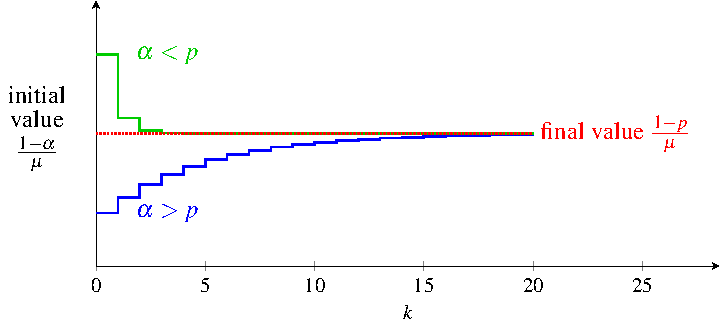
\includegraphics[width=0.55\columnwidth]{./Unit-06/img/ControlStepResponses-1.pdf}
       \end{center}
 \item The analysis we carried out, provides \TC{dynamic} actuator sizing clues:
       \begin{itemize}[<+-| alert@+>]
       \item to sustain \TC{steady state}, must be capable of exerting $u_{max}=\frac{1-p}{\mu} w_{max}$;
       \item if control has to \TC{accelerate} the system ($\alpha<p$) must transiently exert\\
             the \TC{larger} value $u_{max}=\frac{1-\alpha}{\mu} w_{max}$.
       \end{itemize}
 \item Analogous considerations based on the maximum amplitude of $d$,\\
       and the required speed for its rejection, are left as a simple exercise.
 \end{itemize}
\end{frame}

\begin{frame}
\frametitleTC{Pure DT case}
\framesubtitleTC{One-step delayed integrator}
\myPause
 \begin{itemize}[<+-| alert@+>]
 \item A process structure quite frequently encountered in computer-related controls,\\
       is the \TC{one-step delayed integrator}
       \begin{displaymath}
        P(z) = \frac{\mu}{z-1}.
       \end{displaymath}
 \item The name is motivated by the time-domain formulation
       \begin{displaymath}
        y(k) = y(k-1) + \mu u(k-1),
       \end{displaymath}
       showing that at step $k$, $y$ is the sum (DT integral) of $\mu u$ up to the\\
       previous step $k-1$.
 \end{itemize}
\end{frame}

\begin{frame}
\frametitleTC{Pure DT case}
\framesubtitleTC{One-step delayed integrator}
\myPause
 \begin{itemize}[<+-| alert@+>]
 \item If we apply the same policy we used for the stable asymptotically case just setting $p=1$, we get
       \begin{displaymath}
        \begin{array}{l}
          P(z)              = \frac{\mu}{z-1} \\
          G_{yw}^{\circ}(z) = \frac{1-\alpha}{z-\alpha}
          \text{ or }
          G_{yd}^{\circ}(z) = \frac{z-1}{z-\alpha}       
        \end{array}
        \quad \Rightarrow \quad
        C_{PI}(z)  = K\,\frac{z-\zeta}{z-1}, \quad
        K          = \frac{1-\alpha}{\mu}, \;
        \red{\zeta = 1}.
       \end{displaymath}
 \item But we are NOT realising a controller with \red{a zero/pole cancellation on the circle},\\
       as this would create a non asymptotically stable hidden part in the closed-loop\\
       system.
\item Hence we only use the P controller
       \begin{displaymath}
        C(z) = \frac{1-\alpha}{\mu}.
       \end{displaymath}
      and we are back to the case we already treated.
 \end{itemize}
\end{frame}

\begin{frame}[fragile]
\frametitleTC{Sampled-signal case}
\framesubtitleTC{Dominantly first-order asymptotically stable process}
\myPause
 \begin{itemize}[<+-| alert@+>]
 \item Just a bit of CT: if we take the first-order LTI system
       \begin{displaymath}
        \dot{y}(t) = ay(t)+bu(t)
       \end{displaymath}
 \item and set $y(0)=0$, $u(t)=1$ for $t \geq 0$ to compute its unit step response, we get
       \begin{displaymath}
        y(t) = \frac{b}{a} \left( e^{at}-1 \right)
       \end{displaymath}
 \item Check (wxMaxima):
       \begin{verbatim}
  y: b/a*(exp(a*t)-1);
  u: 1;
  ratsimp(diff(y,t)-(a*y+b*u)); /* -> zero, OK */
  subst(t=0,y);                 /* -> zero, OK */
       \end{verbatim}
 \end{itemize}
\end{frame}

\begin{frame}
\frametitleTC{Sampled-signal case}
\framesubtitleTC{Dominantly first-order asymptotically stable process}
\myPause
 \begin{itemize}[<+-| alert@+>]
 \item Incidentally, the response converges for $a<0$ (system asymptotically stable),\\
       is constant for $a=0$ (simply stable) and diverges for $a>0$ (unstable).
 \item Generalising to orders above one, there is a stability theorem for CT systems\\
       identical to the one we know for DT ones, if not for replacing ``magnitude\\
       of eigenvalue of $A$ $\lesseqgtr$ 1'' with ``real part of eigenvalue of $A$ $\lesseqgtr$ 0''.\\
 \item Enough for us here.
 \end{itemize}
\end{frame}

\begin{frame}
\frametitleTC{Sampled-signal case}
\framesubtitleTC{Dominantly first-order asymptotically stable process}
\myPause
 \begin{itemize}[<+-| alert@+>]
 \item If we re-write the CT system above with differently named parameters, i.e.,
       \begin{displaymath}
        \dot{y}(t) = -\frac{1}{T}y(t) + \frac{\mu}{T} u(t)
       \end{displaymath}
 \item[] where asymptotic stability means $T>0$, the unit step response takes the form
       \begin{displaymath}
        y(t) = \mu \left( 1-e^{-t/T} \right).
       \end{displaymath}
 \item Taking also $\mu>0$ for simplicity and without loss of generality,\\
       we can READ the system parameters on a step response plot.
 \end{itemize}
\end{frame}

\begin{frame}
\frametitleTC{Sampled-signal case}
\framesubtitleTC{Dominantly first-order asymptotically stable process}
\myPause
 \begin{center}
  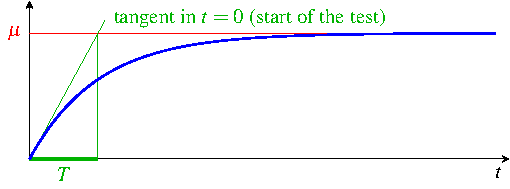
\includegraphics[width=0.55\columnwidth]{./Unit-06/img/FOstepResponse.pdf}
 \end{center}
 \begin{itemize}[<+-| alert@+>]
 \item \vspace{-4mm}When you know nothing about the system you need to control, but you know\\
       what is the input and what is the output, a viable way to get a model,\\
       is to perform a \TC{step test}.
 \item If the response resembles the first-order one above, you can read $\mu$\\
       and $T$ on the response record.
 \item Recall however that the $t$ axis is a CT one: seconds, minutes,...\\
       NOT samples, we still have to decide $T_s$ for our control.
 \end{itemize}
\end{frame}

\begin{frame}[label={pag:FOsystem-DT}]
\frametitleTC{Sampled-signal case}
\framesubtitleTC{Dominantly first-order asymptotically stable process}
\myPause
 \begin{itemize}[<+-| alert@+>]
 \item Now let us turn the system to DT as we already did:
       \begin{displaymath}
        \dot{y}(t) = -\frac{1}{T}y(t) + \frac{\mu}{T} u(t) \quad \Rightarrow \quad
        \frac{y(k)-y(k-1)}{T_s} = -\frac{1}{T}y(k) + \frac{\mu}{T} u(k). 
       \end{displaymath}
 \item This allows us to compute the DT transfer function as
       \begin{displaymath}
        \frac{1-z^{-1}{T_s}}y(k) = -\frac{1}{T}y(k) + \frac{\mu}{T} u(k) \; \Rightarrow \;
        P(z) = \frac{y(k)}{u(k)} = \frac{\mu\frac{T_s}{T+T_s}z}{z-\frac{T}{T+T_s}}.
       \end{displaymath}
 \item Quite expectedly, we have a first-order DT system whose parameters\\
       depend on $T_s$, i.e.,
       \begin{displaymath}
        P(z) = \frac{\rho z}{z-p}, \qquad
        \rho = \mu\frac{T_s}{T+T_s}, \quad
        p    = \frac{T}{T+T_s}.
       \end{displaymath}
 \end{itemize}
\end{frame}

\begin{frame}
\frametitleTC{Sampled-signal case}
\framesubtitleTC{Dominantly first-order asymptotically stable process}
\myPause
 \begin{itemize}[<+-| alert@+>]
 \item Results for different values of $T_s$ versus the CT case (dash-dot line):
       \begin{center}
        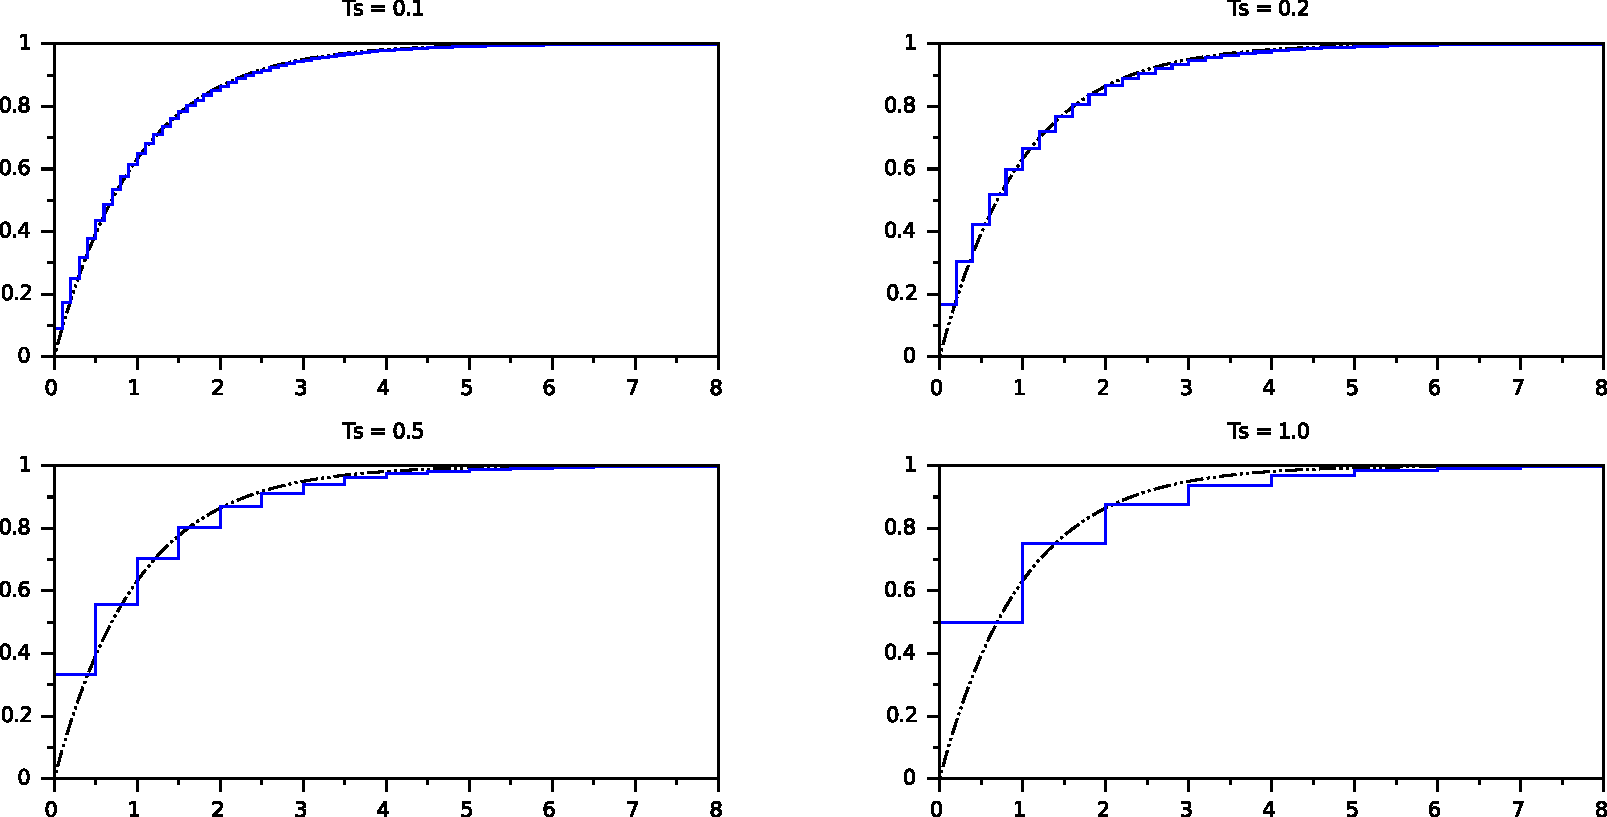
\includegraphics[width=0.60\columnwidth]{./Unit-06/img/CTvsDTexample-step.pdf}
       \end{center}
 \item \TC{Rule of thumb} to select $T_s$ for a representative DT approximation:\\
       at most 1/5 of $T$ (in our case $T=1$, $T_s=0.2$ is fine).
 \item Plenty of theory omitted, if interested ask for references...
 \end{itemize}
\end{frame}

\begin{frame}
\frametitleTC{A CT interpretation of the PI law}
\framesubtitleTC{useful for tuning}
\myPause
 \begin{itemize}[<+-| alert@+>]
 \item Can we interpret the PI control law
       \begin{displaymath}
        C_{PI}(z) = K \frac{z-\zeta}{z-1}
       \end{displaymath}
       in the continuous time, so as to derive $T_s$-independent parameters for it as well?
 \item Of course. To this end, let us split the P and the I action again.
 \item The P action has no dynamics, for it the DT and the CT domains\\
       are the same:
       \begin{displaymath}
        u_P(k) = K_P e(k), \quad
        u_P(t) = K_P e(t).
       \end{displaymath}
 \end{itemize}
\end{frame}

\begin{frame}
\frametitleTC{A CT interpretation of the PI law}
\framesubtitleTC{}
\myPause
 \begin{itemize}[<+-| alert@+>]
 \item The integral action in the CT domain is conversely a true integral:
       \begin{displaymath}
        u_I(t) = K_I \int_0^t e(\tau)d\tau.
       \end{displaymath}
 \item As an immediate consequence, then,
       \begin{displaymath}
        \dot{u}_I(t) = K_I e(t),
       \end{displaymath}
 \item and once again, we relate CT to DT by replacing the time derivative\\
       with the incremental ratio over one step of length $T_s$, which yields
       \begin{displaymath}
        \frac{u_I(k)-u_I(k-1)}{T_s}= K_I e(k).
       \end{displaymath}
 \end{itemize}
\end{frame}

\begin{frame}
\frametitleTC{A CT interpretation of the PI law}
\framesubtitleTC{}
\myPause
 \begin{itemize}[<+-| alert@+>]
 \item It is a convention of the PI(D) literature and practice to express $K_I$ as the\\
       proportional control gain divided by a time, which is dimensionally consistent,\\
       i.e., to write in the CT
       \begin{displaymath}
        u_P(t)       = K e(t), \quad
        \dot{u}_I(t) = \frac{K}{T_i} e(t)
       \end{displaymath}
       where $K$ is called (somehow improperly) the \TC{gain}, and $T_i$ the \TC{integral time}.
 \item This reflects in the DT controller
       \begin{displaymath}
        \begin{array}{rcl}
         u_P(k) &=& K e(k) \\
         u_I(k) &=& u_I(k-1) + \frac{KT_s}{T_i} e(k)
        \end{array}
       \end{displaymath}
 \item In transfer function form, then,
       {\small
       \begin{displaymath}
        C_{PI}(z) = \frac{u_P(k)+u_I(k)}{e(k)}
                  = K + \frac{zKT_s}{T_i(z-1)}
                  = \frac{K(T_i+T_s)}{T_i} \, \frac{z-\frac{T_i}{T_i+T_s}}{z-1}.
       \end{displaymath}
       }
 \end{itemize}
\end{frame}

\begin{frame}
\frametitleTC{A CT interpretation of PI and 1st order model}
\framesubtitleTC{again in a view to controller tuning}
\myPause
 \begin{itemize}[<+-| alert@+>]
 \item Let us look at the first-order process model and the PI controller, once their\\
       $T_s$-independent parameters -- $(\mu,T)$ for $P$, $(K,T_i)$ for $C$ -- are evidenced:
       \begin{displaymath}
        P(z)      = \mu \frac{\frac{T_s}{T+T_s} z}{z-\frac{T}{T+T_s}}, \qquad
        C_{PI}(z) = \frac{K(T_i+T_s)}{T_i} \, \frac{z-\frac{T_i}{T_i+T_s}}{z-1}.
       \end{displaymath}
 \item Since $T>0$ by hypothesis and so is obviously $T_s$ as well, the process pole\\
       is within the unit circle.
 \item We can therefore tune the PI by cancellation, but now to do this we\\
       set $T_i=T$, i.e., \TC{we operate in the CT domain}. Doing so produces 
       \begin{displaymath}
        L(z) = \mu \frac{\frac{T_s}{\ccancel[green]{T+T_s}} z}{\ccancel[red]{z-\frac{T}{T+T_s}}}
               \frac{K\ccancel[green]{(T+T_s)}}{T} \, \frac{\ccancel[red]{z-\frac{T}{T+T_s}}}{z-1}
             = \frac{\mu K T_s}{T} \frac{z}{z-1}.
       \end{displaymath}
 \end{itemize}
\end{frame}

\begin{frame}
\frametitleTC{A CT interpretation of control objectives}
\framesubtitleTC{}
\myPause
 \begin{center}
  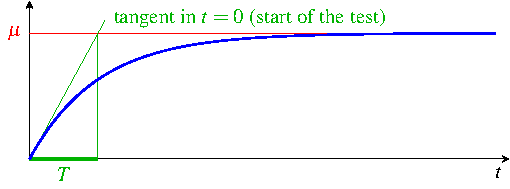
\includegraphics[width=0.45\columnwidth]{./Unit-06/img/FOstepResponse.pdf}
 \end{center}
 \begin{itemize}[<+-| alert@+>]
 \item If we want $y$ to reach $u$ within a certain time, the $y \rightarrow w$ continuous time system\\
       has to share the structure of the first-order process, but with $\mu=1$\\
       and a value of $T$ reflecting the desired speed.
 \item Since in the response above $y$ reaches its final value in about $5T$,\\
       if we want the closed-loop system to make $y$ reach $w$ and settle\\
       in a time $t_{set}$, then the required $T$ is $t_{set}/5$. Let us call this quantity\\
       $\lambda$ for brevity.
 \end{itemize}
\end{frame}

\begin{frame}[fragile]
\frametitleTC{Joining the pieces}
\framesubtitleTC{to the purpose of tuning}
\myPause
 \begin{itemize}[<+-| alert@+>]
 \item Substituting $\mu=1$ and $T=\lambda$ in the expression we found above for $P(z),$\\
       we get the objective $y/w$ transfer function as
       \begin{displaymath}
        G_{yw}^{\circ}(z) = \frac{\frac{T_s}{\lambda+T_s} z}{z-\frac{\lambda}{\lambda+T_s}}, \quad
        \lambda           = \frac{t_{set}}{5}
       \end{displaymath}
 \item We can then apply direct synthesis (wxMaxima):
       \begin{verbatim}
  P   : mu*Ts/(T+Ts)*z/(z-T/(T+Ts));
  Gywo: Ts/(lambda+Ts)*z/(z-lambda/(lambda+Ts));
  Csol: rhs(solve(P*C/(1+P*C)=Gywo,C)[1]);
       \end{verbatim}
 \end{itemize}
\end{frame}

\begin{frame}[fragile,label={pag:PItuning-lambda}]
\frametitleTC{Tuning}
\framesubtitleTC{direct synthesis for set point tracking -- CT setting}
\myPause
 \begin{itemize}[<+-| alert@+>]
 \item The result corresponds to the expression we already found for $C$, with
       \begin{displaymath}
        K   = \frac{T}{\lambda\mu}, \quad
        T_i = T.
       \end{displaymath}
 \item check (wxMaxima):
       {\small
       \begin{verbatim}
  K   : T/(mu*lambda);
  Ti  : T;
  Cchk: K*(Ti+Ts)/Ti*(z-Ti/(Ti+Ts))/(z-1); /* The C we got */
  ratsimp(Cchk-Csol);                      /* -> zero, OK  */
       \end{verbatim}
       }
 \item The ``direct synthesis for disturbance rejection'' case is left as a\\
       simple exercise (use wxMaxima). We now observe our result to\\
       make some important remarks.
 \end{itemize}
\end{frame}

\begin{frame}
\frametitleTC{Remarks}
\framesubtitleTC{direct synthesis for set point tracking -- CT setting}
\myPause
 \begin{itemize}[<+-| alert@+>]
 \item We showed that the idea of tuning by cancellation can be somehow applied\\
       in the CT domain as well.
 \item We have to say ``somehow'' because we do not possess the knowledge of\\
       \TC{CT transfer function}.
 \item Such an object can be defined, however, and the DT theory we saw can be\\
       completed with its CT counterpart.
 \item In fact, just to notice, the CT side of the matter was born far before.
 \end{itemize}
\end{frame}

\begin{frame}
\frametitleTC{Remarks}
\framesubtitleTC{general ideas to remember}
\myPause
 \begin{itemize}[<+-| alert@+>]
 \item You can derive a ``model for control'' that is VERY SIMPLE, yet enough\\
       for tuning, even just by looking at recorded data.
 \item So simple models are often flagged as ``too simple to provide realistic\\
       guarantees''...
 \item ...but basically by researchers who do not know about the Systems and Control\\
       Theory (no judgement, just mentioning facts).
 \item Be careful about ``realism'', and always consider the PURPOSE of\\
       your model.
 \item In the end, for example, temperature is molecular motion, but luckily\\
       we do not need to follow individual molecules to do temperature\\
       control \smiley.
 \end{itemize}
\end{frame}

\begin{frame}
\frametitleTC{Remarks}
\framesubtitleTC{General ideas to remember}
\myPause
 \begin{itemize}[<+-| alert@+>]
 \item On the symmetric front, be careful about the REPRESENTATIVENESS\\
       of your model.
 \item If you have knowledge of the phenomenon, that is a great advantage.
 \item If you need to rely on data, be sure to explore all the relevant dynamics.
 \item Experiment design is itself a discipline, explore it and/or get in touch with\\
       experts of the Identification Theory.
 \item And in general, be cautious about benchmarks that assert they are ``general''\\
       just because e.g. they contain a ``large'' number of ``heterogeneous''\\
       applications.
 \item By themselves, such statements provide NO guarantee that the\\
       tuned control will not have to face a totally unforeseen dynamics.
 \end{itemize}
\end{frame}

\begin{frame}
\frametitleTC{Remarks}
\framesubtitleTC{Even more general ideas to remember}
\myPause
 \begin{itemize}[<+-| alert@+>]
 \item To set up a control \TC{you need a model}.
 \item A model for that purpose is a \TC{dynamic system}.
 \item If you need formal guarantees on control, you need the Systems Theory.
 \item []{\small
       \begin{quote}
        There is no royal road to geometry.\\
        \vspace{1mm}\hspace{70mm}Euclid
       \end{quote}
       }
 \item However, never stretch a model beyond its purpose.
 \item []{\small
       \begin{quote}
        Since all models are wrong the scientist cannot obtain a ``correct'' one\\
        by excessive elaboration. On the contrary following William of Occam\\
        he should seek an economical description of natural phenomena.\\
        Just as the ability to devise simple but evocative models\\
        is the signature of the great scientist so overelaboration\\
        and overparameterization is often the mark of mediocrity.\\
        \vspace{1mm}\hspace{70mm}George Box
       \end{quote}
       }
 \item []...often summarised as ``all models are wrong, some are useful''. 
 \end{itemize}
\end{frame}

\section{The PID control law}
\subsection{}

\begin{frame}
\frametitleTC{The overall law}
\framesubtitleTC{recap in preparation for the implementation}
\myPause
 \begin{itemize}[<+-| alert@+>]
 \item The control signal $u(k)$ is the sum of the Proportional (P), the Integral (I)\\
       and the derivative (D) action:
       \begin{displaymath}
        u(k) = u_P(k)+u_I(k)+u_D(k).
       \end{displaymath}
 \item Some action may not be present, giving rise to the P, I, PI, PD laws -- with\\
       obvious meaning -- besides the complete PID one (D and ID make little\\
       -- if any -- sense in practice, we omit further discussions).
 \item We shall now study the three actions, then deal with actuator limits,\\
       and finally move to the algorithm.
 \end{itemize}
\end{frame}

\begin{frame}
\frametitleTC{The P action}
\framesubtitleTC{}
\myPause
 \begin{itemize}[<+-| alert@+>]
 \item The P action $u_P(k)$ is computed as
       \begin{displaymath}
        u_P(k) = K e(k).
       \end{displaymath}
 \item Its role is to respond \TC{promptly} to an error variation.
 \item Since there is no dynamics, that response is in fact instantaneous\\
       (if not for computation delay and machine-related timing facts\\
       at large).
 \end{itemize}
\end{frame}

\begin{frame}
\frametitleTC{The I action}
\framesubtitleTC{}
\myPause
 \begin{itemize}[<+-| alert@+>]
 \item The I action $u_I(k)$ is computed as
       \begin{displaymath}
        u_I(k) = u_I(k-1) + \frac{KT_s}{T_i} e(k).
       \end{displaymath}
 \item Its role is to guarantee \TC{zero steady-state error}.
 \item At steady state everything (including $u_I$) is constant, and therefore\\
       the error must be zero because in the opposite case $u_I$ would vary.
 \item In general, if your control scheme has to ensure that some variable\\
       is zero at steady state, just make that variable the input of an\\
       integrator. 
 \end{itemize}
\end{frame}

\begin{frame}
\frametitleTC{The D action}
\framesubtitleTC{}
\myPause
 \begin{itemize}[<+-| alert@+>]
 \item The D action \TC{in the CT domain} is expressed as
       \begin{displaymath}
        u_D(t) = K T_d \frac{de(t)}{dt}
       \end{displaymath}
       where $T_d$ is called the \TC{derivative time}.
 \item Its role is to attempt to \TC{anticipate the error} over a horizon $T_d$ in the future.
 \item Interpretation (and \emph{caveat} to not make $T_d$ too large):
       \begin{center}
        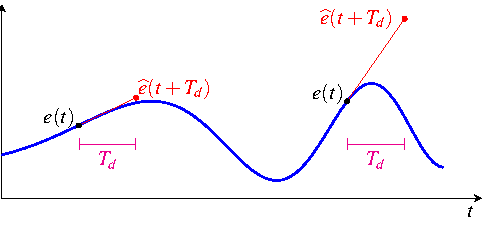
\includegraphics[width=0.45\columnwidth]{./Unit-06/img/D-action-interpretation.pdf}
       \end{center}
 \end{itemize}
\end{frame}

\begin{frame}
\frametitleTC{The D action}
\framesubtitleTC{}
\myPause
 \begin{itemize}[<+-| alert@+>]
 \item Sometimes the D action may respond too nervously, and therefore it is in fact computed as
       \begin{displaymath}
        u_D(k) = \beta u_D(k-1) + (1-\beta) K T_d \frac{e(k)-e(k-1)}{Ts}, \quad 0 < \beta < 1.
       \end{displaymath}
 \item In this course we provide no notion of \TC{frequency response} -- another hook for the\\
       interested -- but it should be intuitive that if $u_D(k)$ contains a fraction\\
       $\beta$ of $u_D(k-1)$ while the new input's contribution only weighs $1-\beta$,\\
       this combination acts as a \TC{lowpass filter}, i.e., smooths out the abrupt\\
       variations of $u_D$ that the input would otherwise provoke.
 \item In $z$ form we thus have
       \begin{displaymath}
        \frac{u_D(k)}{e(k)} = \frac{1-\beta}{z-\beta} \frac{K T_d}{T_s} \frac{z-1}{z}.
       \end{displaymath}
 \end{itemize}
\end{frame}

\begin{frame}
\frametitleTC{The D action}
\framesubtitleTC{}
\myPause
 \begin{itemize}[<+-| alert@+>]
 \item For reasons we do not have the time to fully discuss here (but ask if interested)\\
       it is convenient to set
       \begin{displaymath}
        \beta = \frac{T_d}{T_d+NT_s}, \qquad N>0,
       \end{displaymath}
       in a nutshell because doing so
       \begin{itemize}[<+-| alert@+>]
       \item the pole $\beta$ of the $u_D/e$ transfer function is surely in the range $(0,1)$,
       \item if $T_d=0$ (PI only) $\beta$ vanishes as well,
       \item parameter $N$ is a good knob to control the amount of smoothing applied\\
             to $u_D$ (higher $N$ means lower $\beta$, thus less of $u_D(k-1)$ in $u_D(k)$, thus\\
             less smoothing --- and clearly \textit{vice versa}). 
       \end{itemize}
 \item We are now ready for a PID ``quasi-algorithm''.
 \item In fact now we write just the essentials and then, after discussing\\
       control limits, we get to the real thing, also introducing some\\
       practically useful additions.
 \end{itemize}
\end{frame}

\begin{frame}[fragile,label={pag:PID-quasi-alg}]
\frametitleTC{A PID quasi-algorithm}
\framesubtitleTC{to be executed periodically with timestep $T_s$}
\myPause
 \begin{verbatim}
  e      = w-y;
  up     = K*e;
  ui     = ui_old+K*Ts/Ti*e;
  ud     = beta*ud_old+(1-beta)*K*Td/Ts*(e-e_old);
  u      = up+ui+ud;
  e_old  = e;
  ui_old = ui;
  ud_old = ud;
 \end{verbatim}
\end{frame}


\section{The control algorithm}
\subsection{}

\begin{frame}
\frametitleTC{Actuator limits}
\framesubtitleTC{}
\myPause
 \begin{itemize}[<+-| alert@+>]
 \item No physical signal can go from $-\infty$ to $\infty$.
 \item Hence control signals are invariably subject to \TC{saturation}.
 \item Modelling the relationship between a non saturated control $u_{ns}$ and the quantity $u$\\
       really exerted by an actuator with limits $(u_{min},u_{max})$ is trivial:
       \begin{displaymath}
        u(k) = \max \bigg( u_{min}, \min \big( u_{max}, u_{ns}(k) \big) \bigg).
       \end{displaymath}
 \item The point is that \TC{in the presence of a dynamic controller}, just\\
       clamping the output can make this inconsistent with the state,\\
       leading to a phenomenon called \TC{windup}. 
 \end{itemize}
\end{frame}

\begin{frame}
\frametitleTC{Windup}
\framesubtitleTC{Example with a PI}
\myPause
 \begin{columns}
  \column[T]{0.40\textwidth}
   \only<2->{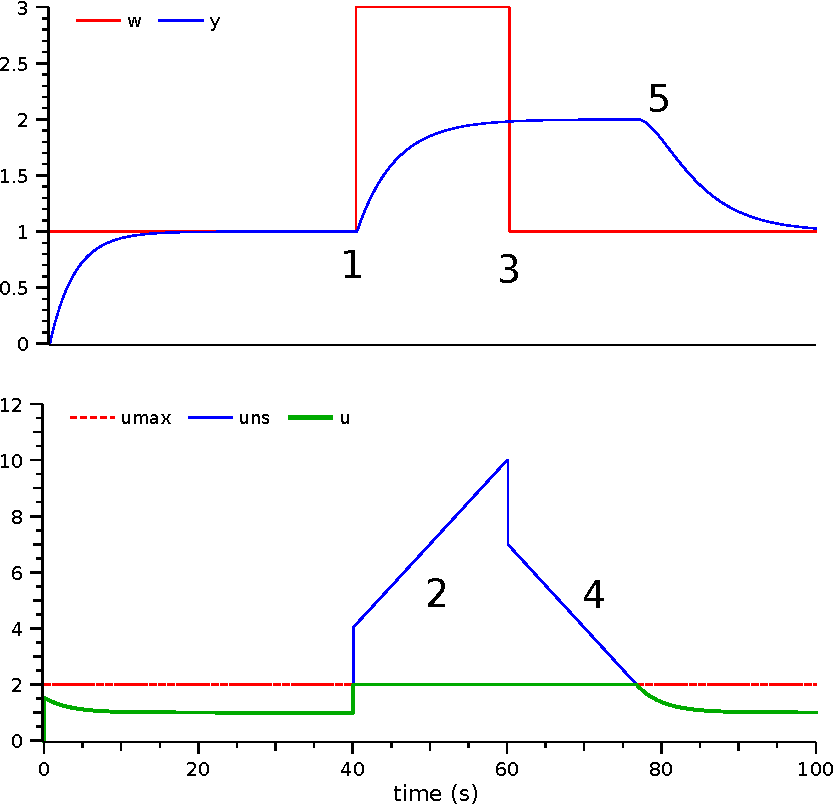
\includegraphics[height=6cm]{./Unit-06/img/example-windup-wy-u.pdf}}
  \column[T]{0.60\textwidth}
  \myPause
   \begin{itemize}[<+-| alert@+>]
   \item[1] $w$ is set to a value that cannot be obtained\\
            owing to actuator limits;
   \item[2] the really exerted $u$ stops at $u_{max}$, but as $e>0$,\\
            the computed $u_{ns}$ keeps growing due to the\\
            I action;
   \item[3] $w$ is led back to an attainable value...
   \item[4] ...but $u$ is stuck at $u_{max}$ until $u_{ns}$\\
            decreases below it, which takes\\
            some time,
   \item[5] hence $y$ remains stuck as well,\\
            and this is \TC{windup}.
   \end{itemize}
 \end{columns}
\end{frame}

\begin{frame}
\frametitleTC{Windup}
\framesubtitleTC{An important remark}
\myPause
 \begin{itemize}[<+-| alert@+>]
 \item Given its origin in a controller with I action, several texts call the phenomenon\\
       ``\underline{integral} windup''.
 \item This may be misleading, in that one may think that in the absence of I action,\\
       \TC{antiwindup} -- that we are introducing shortly -- is not necessary.
 \item WRONG. \underline{Any} \TC{dynamic} controller can generate windup: it suffices that the\\
       controller output is clamped, and the controller state is not made consistent\\
       with the clamped value.
 \item \vfill Incidentally, we just saw one possible way of realising antiwindup. 
 \end{itemize}
\end{frame}

\begin{frame}
\frametitleTC{Tracking}
\framesubtitleTC{}
\myPause
 \begin{itemize}[<+-| alert@+>]
 \item In some cases, it may be useful to constrain the controller output to track\\
       a certain signal, fed to the same controller as input.
 \item This is called the \TC{tracking} mode as opposite to the \TC{automatic} mode, in which\\
       the control law is applied normally to compute $u$.
 \item One reason for tracking can be to provide manual control, for example.
 \item In tracking mode, the state of the controller must be made consistent with the\\
       prescribed output; otherwise, when switching back to automatic mode,\\
       the first $u$ would come from the present $e$ and from the state\\
       computed the last time the controller was in automatic, in general\\
       causing an undesired transient. 
 \end{itemize}
\end{frame}

\begin{frame}
\frametitleTC{Tracking}
\framesubtitleTC{}
\myPause
 \begin{itemize}[<+-| alert@+>]
 \item Tracking is activated by a logical input generally called TS (\TC{Track Switch}):
       \begin{itemize}[<+-| alert@+>]
       \item when TS is false, $u$ is computed by the control law;
       \item when TS is true, $u$ is set equal to the value of a numeric controller input\\
             generally called TR (\TC{Track Reference}). 
        \end{itemize}
 \item We are now seeing antiwindup and tracking realised, by going through\\
       a complete PI algorithm.
 \end{itemize}
\end{frame}

\begin{frame}[fragile,label={pag:PI-complete-alg}]
\frametitleTC{A complete algorithm}
\framesubtitleTC{PI case to comment in detail}
\myPause
 {\scriptsize
 \begin{verbatim}
 e      = w-y;                   // Compute error
 up     = K*e;                   // P action needed irrespectively of the mode, see (*) below
 if not TS then                  // Automatic mode, compute I action and then u
    ui  = ui_old+K*Ts/Ti*e;
    u   = up+ui;
 else                            // Tracking mode, set u equal to TR
    u   = TR;
 end if;
 u      = max(umin,min(umax,u)); // Apply control limits
 ui_old = u-up;                  // Make state ui_old for next run consistent with u and e (*)
 \end{verbatim}
 }\myPause
 \vspace{-3mm}\begin{itemize}[<+-| alert@+>]
 \item The last line is the state management for antiwindup and tracking.
 \item This is the PI code we shall realise in Modelica: notice compactness\\
       and readability (if one knows the theory behind).
 \item If needed, porting to C, C++, fortran, java, python, whatever,\\
       is clearly straightforward. 
 \end{itemize}
\end{frame}

\begin{frame}[fragile]
\frametitleTC{A complete algorithm}
\framesubtitleTC{PID case -- study at home, ask questions next time if needed}
\myPause
 {\scriptsize
 \begin{verbatim}
 e         = w-y;
 up        = K*e;
 if not TS then
    ui     = ui_old+K*Ts/Ti*e;
    ud     = beta*ud_old+(1-beta)*K*Td/Ts*(e-e_old);
    u      = up+ui;
 else
    u      = TR;
    ud     = 0;                                      // (1) Why the arbitrary choice ud=0 here?
 end if;
 u         = max(umin,min(umax,u));
 ui_old    = u-up;
 if u>= umax or u<= umin then                        // (2) Why when u is clamped
    ud_old = 0;                                      //     ud_old for next run
 else                                                //     is set to zero
    ud_old = ud;                                     //     as well?
 end if;
 \end{verbatim}
 }\myPause
 \vspace{-6mm}\begin{itemize}[<+-| alert@+>]
 \item Suggestion for \texttt{(1)} and \texttt{(2)}: consider the relative entity of the P, I,\\
       and D actions...
 \end{itemize}
\end{frame}


\section{Conclusions}
\subsection{}

\begin{frame}
\frametitleTC{Conclusions}
\framesubtitleTC{Recap and lessons learnt (1/2)}
\myPause
 \begin{itemize}[<+-| alert@+>]
 \item We can characerise a dynamic system with \TC{time domain responses}.
 \item These refer to a certain \emph{stimulus} (we used impulse and step).
 \item Responses can be used also to stipulate \TC{control objectives}.
 \item A viable way to do so is to transform time domain deires into some desired
       closed-loop transfer function.
 \item This paves the way to the \TC{direct synthesis} technique.
 \end{itemize}
\end{frame}

\begin{frame}
\frametitleTC{Conclusions}
\framesubtitleTC{Recap and lessons learnt (2/2)}
\myPause
 \begin{itemize}[<+-| alert@+>]
 \item We have open issues, however.
       \begin{itemize}[<+-| alert@+>]
       \item Why impulse and step \emph{stimuli} are meaningful?
       \item How can we choose the target closed-loop transfer function?
       \item What are the limits and what is their origin?
       \end{itemize}
 \item \vfill These issues are very suited for addressing in a practice session,\\
       which is our next task.
 \item Please review your notes, next time ask questions if needed\\
       before we start.
 \end{itemize}
\end{frame}

\section{}
{
\setbeamertemplate{headline}{
  \begin{beamercolorbox}[wd=\paperwidth,ht=4.2ex,dp=1.5ex]{palette quaternary}
  \end{beamercolorbox}
  }
\setbeamertemplate{footline}{
  \begin{beamercolorbox}[wd=\paperwidth,ht=2.2ex,dp=1.5ex]{palette quaternary}
  \end{beamercolorbox}
  }
\begin{frame}[noframenumbering]
 \vspace{20mm}\Huge{Discussion open}
\end{frame}
}


